%
% File acl2010.tex
%
% Contact  jshin@csie.ncnu.edu.tw or pkoehn@inf.ed.ac.uk
%%
%% Based on the style files for ACL-IJCNLP-2009, which were, in turn,
%% based on the style files for EACL-2009 and IJCNLP-2008...

%% Based on the style files for EACL 2006 by 
%%e.agirre@ehu.es or Sergi.Balari@uab.es
%% and that of ACL 08 by Joakim Nivre and Noah Smith

\documentclass[11pt]{article}
\usepackage{acl2012}
\usepackage{times}
\usepackage{float}
\usepackage{url}
\usepackage{latexsym}
\usepackage{epsfig}
\usepackage{subfig}    
\usepackage{latexsym}
\usepackage[usenames]{color}
\usepackage{times} 
\usepackage{verbatim}
\usepackage{multirow}
\usepackage{threeparttable}
\usepackage{booktabs}
\usepackage{mdwlist}
%\setlength\titlebox{6.5cm}    % You can expand the title box if you
% really have to

\title{Exploring Topic Coherence over many models and many topics}

\author{Keith Stevens$^{1,2}$ 
        Philip Kegelmeyer$^{3}$
        David Andrzejewski$^{2}$
        David Buttler$^{2}$ \\
  $^{1}$University of California Los Angeles; Los Angeles , California, USA \\
  $^{2}$Lawrence Livermore National Lab; Livermore, California, USA \\
  $^{3}$Sandia National Lab; Livermore, California, USA \\
  {\tt \{stevens35,andrzejewski1,buttler1\}@llnl.gov} \\
  {\tt wpk@sandia.gov}
}
 
\date{}

\begin{document}
\maketitle
\begin{abstract}
We apply two new automated semantic evaluations to three distinct latent topic
models.  Both metrics have been shown to align with human evaluations and
provide a balance between internal measures of information gain and comparisons
to human ratings of coherent topics.  We improve upon the measures by
introducing new aggregate measures that allows for comparing complete topic
models.  We further compare the automated measures to other metrics for topic
models, comparison to manually crafted semantic tests and document
classification.  Our experiments reveal that LDA and LSA each have different
strengths; LDA best learns descriptive topics while LSA is best at creating a
compact semantic representation of documents and words in a corpus. 
\end{abstract}

\section{Introduction}
\label{sec:introduction}
Topic models learn bags of related words from large corpora without any
supervision. Based on the words used within a document, they mine topic level
relations by assuming that a single document covers a small set of concise
topics.  Once learned, these topics often correlate well with human concepts.
For example, one model might produce topics that cover ideas such as government
affairs, sports, and movies.  With these unsupervised methods, we can extract 
useful semantic information in a variety of tasks that depend on identifying
unique topics or concepts, such as distributional semantics
\cite{jurgens10sspace}, word sense induction
\cite{vandeCruys11latentWsi,brody09ldawsi}, and information retrieval
\cite{andrzejewski11ldaIR}.  

When using a topic model, we are primarily concerned with the degree to which
the learned topics match human judgments and help us differentiate between
ideas.  But until recently, the evaluation of these models has been ad hoc and
application specific.  Evaluations have ranged from fully automated intrinsic
evaluations to manually crafted extrinsic evaluations.  Previous extrinsic
evaluations have used the learned topics to compactly represent a small fixed
vocabulary and compared this distributional space to human judgments of
similarity \cite{jurgens10sspace}.  But these evaluations are hand constructed
and often costly to perform for domain-specific topics.  Conversely, intrinsic
measures have evaluated the amount of information encoded by the topics, where 
perplexity is one common example\cite{wallach2009evaluation}, however, \newcite{gerrish09tealeaves}
found that these intrinsic measures do not always correlate with semantically
interpretable topics.  Furthermore, few evaluations have used the same metrics
to compare distinct approaches such as Latent Dirichlet Allocation (LDA)
\cite{blei03lda},  Latent Semantic Analysis (LSA) \cite{landauer97solution}, and
Non-negative Matrix Factorization (NMF) \cite{Lee00algorithmsfor}.  This has
made it difficult to know which method is most useful for a given application,
or in terms of extracting useful topics.

We now provide a comprehensive and automated evaluation of these three distinct
models (LDA, LSA, NMF), for automatically learning semantic topics.  While these
models have seen significant improvements, they still represent the core
differences between each approach to modeling topics.  For our evaluation, we
use two recent automated coherence measures \cite{mimno11umass,newman10uci}
originally designed for LDA that bridge the gap between comparisons to
human judgments and intrinsic measures such as perplexity.  We consider several
key questions:
\begin{enumerate*}
{\footnotesize
 \item How many topics should be learned?
 \item How many learned topics are useful?
 \item How do these topics relate to often used semantic tests?
 \item How well do these topics identify similar documents?
 }
\end{enumerate*}

We begin by summarizing the three topic models and highlighting their key
differences.  We then describe the two metrics.  Afterwards, we focus on a
series of experiments that address our four key questions and finally conclude
with some overall remarks.



\section{Topic Models}
\label{sec:topic-models}

We evaluate three latent factor models that have seen widespread usage:
\begin{enumerate*}
{\small
  \item Latent Dirichlet Allocation
  \item Latent Semantic Analysis with Singular Value Decomposition
  \item Latent Semantic Analysis with Non-negative Matrix Factorization
}
\end{enumerate*}

Each of these models were designed with different goals and are supported
by different statistical theories.  We consider both LSA models as topic models
as they have been used in a variety of similar contexts such as distributional
similarity \cite{jurgens10sspace} and word sense induction
\cite{vandeCruys11latentWsi,brody09ldawsi}.  We evaluate these distinct models
on two shared tasks (1) grouping together similar words while separating
unrelated words and (2) distinguishing between documents focusing on different
concepts.

We distill the different models into a shared representation consisting of two
sets of learned relations: how words interact with topics and how topics
interact with documents.  For a corpus with $\mathcal{D}$ documents and
$\mathcal{V}$ words, we denote these relations in terms of $\mathcal{T}$ topics
as
\begin{description}
\item[(1)] a $\mathcal{V} \times \mathcal{T}$ matrix, $W$, that indicates the strength
each word has in each topic, and
\item[(2)] a $\mathcal{T} \times \mathcal{D}$ matrix, $H$, that indicates the strength each topic
has in each document.  

\end{description}
$\mathcal{T}$ serves as a common parameter to each model.

\subsection{Latent Dirichlet Allocation}

Latent Dirichlet Allocation \cite{blei03lda} learns the relationships
between words, topics, and documents by assuming documents are generated by a
particular probabilistic model.  It first assumes that there are a fixed set of
topics, $\mathcal{T}$ used throughout the corpus, and each topic $z$ is associated with a
multinomial distribution over the vocabulary $\Phi_{z}$, which is drawn from a
Dirichlet prior $Dir(\beta)$.  A given document $D_i$ is then generated by the
following process
\begin{enumerate}
{\small
\item Choose $\Theta_i \sim Dir(\alpha)$, a topic distribution for $D_i$
\item For each word $w_j \in D_i$:
  \begin{enumerate}
  \item Select a topic $z_j \sim \Theta_i$
  \item Select the word $w_j \sim \Phi_{z_j}$
  \end{enumerate}
}
\end{enumerate}
  
In this model, the $\Theta$ distributions represent the probability of each
topic appearing in each document and the $\Phi$ distributions represent the
probability of words being used for each topic.  These two sets of distributions
correspond to our $H$ and $W$ matrices, respectively.  The process above defines
a generative model; given the observed corpus, we use collapsed Gibbs sampling
implementation found in Mallet\footnote{http://mallet.cs.umass.edu/} to infer
the values of the latent variables $\Phi$ and $\Theta$
\cite{griffiths_steyvers04}.  The model relies only on two additional hyper
parameters, $\alpha$ and $\beta$,  that guide the distributions.

\begin{table*}[h!t!b!]
\footnotesize
\center
\begin{tabular}{|cllcc|}
\multicolumn{1}{c}{Model} & Label & Top Words & UMass & \multicolumn{1}{l}{UCI} \\
\hline
\multicolumn{3}{l}{\textbf{High Quality Topics}} \\
\hline
\multirow{2}{*}{LDA} 
% 500-32
& interview & told asked wanted interview people made thought time called knew 
& -2.52 & 1.29 \\
% 500-176
& wine & wine wines bottle grapes made winery cabernet grape pinot red 
& -1.97 & 1.30 \\
\hline
\multirow{2}{*}{NMF} 
% 500-144
& grilling & grilled sweet spicy fried pork dish shrimp menu dishes sauce 
& -1.01 & 1.98 \\
% 500-120
& cloning & embryonic cloned embryo human research stem embryos cell cloning cells
& -1.84 & 1.46 \\
\hline
\multirow{2}{*}{SVD} 
% 500-5
& cooking & sauce food restaurant water oil salt chicken pepper wine cup 
& -1.87 & -1.21 \\
% 500-25
& stocks & fund funds investors weapons stocks mutual stock movie film show 
& -2.30 & -1.88 \\
\hline

\multicolumn{3}{l}{\textbf{Low Quality Topics}} \\
\hline
\multirow{2}{*}{LDA} 
% 500-290
& rates & 10-yr rate 3-month percent 6-month bds bd 30-yr funds robot 
& -1.94 & -12.32 \\
% 500-340
& charity & fund contributions .com family apartment charities rent 22d children assistance
& -2.43 & -8.88 \\
\hline
\multirow{2}{*}{NMF} 
% 500-76
& plants & stem fruitful stems trunk fruiting currants branches fence currant espalier 
& -3.12 & -12.59 \\
% 500-33
& farming & buzzards groundhog prune hoof pruned pruning vines wheelbarrow tree clematis
& -1.90 & -12.56 \\
\hline
\multirow{2}{*}{SVD} 
% 500-7
& city & building city area buildings p.m. floors house listed eat-in a.m.
& -2.70 & -8.03 \\
% 500-160
& time & p.m. system study a.m. office political found school night yesterday 
& -1.67 & -7.02 \\
\hline
\end{tabular}
\caption{Top 10 words from several high and low quality topics when ordered by
the UCI Coherence Measure.  Topic labels were chosen in an ad hoc manner only to
briefly summarize the topic's focus.}
\label{tab:best}
\end{table*}


\subsection{Latent Semantic Analysis}

Latent Semantic Analysis \cite{landauer97solution,landauer98lsa} learns topics
by first forming a traditional term by document matrix used in information
retrieval and then smoothing the counts to enhance the weight of informative
words.  Based on the original LSA model, we use the Log-Entropy transform.  
LSA then decomposes this smoothed, term by document matrix in order to
generalize observed relations between words and documents.  For both LSA models,
we used implementations found in the S-Space
package.\footnote{https://github.com/fozziethebeat/S-Space}

Traditionally, LSA has used the Singular Value Decomposition, but we also
consider Non-negative Matrix Factorization as we've seen NMF applied in similar
situations \cite{pauca04nmfIR} and others have found a connection between NMF
and Probabilistic Latent Semantic Analysis \cite{ding08nmfPlsa}, an extension to
LSA.  We later refer to these two LSA models simply as SVD and NMF to emphasize
the difference in factorization method.

\paragraph{Singular Value Decomposition}
decomposes $M$ into three smaller matrices
$$
M=U \Sigma V^{T}
$$
\noindent
and minimizes Frobenius norm of $M$'s reconstruction error with the constraint
that the rows of $U$ and $V$ are orthonormal eigenvectors.  Interestingly, the
decomposition is agnostic to the number of desired dimensions.  Instead, the
rows and columns in $U$ and $V^T$ are ordered based on their descriptive power,
i.e. how well they remove noise, which is encoded by the diagonal singular value
matrix $\Sigma$.  As such, reduction is done by retaining the first
$\mathcal{T}$ rows and columns from $U$ and $V^T$.  For our generalization, we
use $W=U \Sigma$ and $H = \Sigma V^T$.  We note that values in $U$ and $V^T$ can
be both negative and positive, preventing a straightforward interpretation as
unnormalized probabilities

\paragraph{Non-negative Matrix Factorization}
also factorizes $M$ by minimizing the reconstruction error, but with only one
constraint: the decomposed matrices consist of only non-negative values.
In this respect, we can consider it to be
learning an unnormalized probability distributions over topics.  We use the original
Euclidean least squares definition of NMF\footnote{We note that the
alternative KL-Divergence form of NMF has been directly linked to PLSA
\cite{ding08nmfPlsa}}.  Formally, NMF is defined as

$$M = W H$$
\noindent
where $H$ and $W$ map directly onto our generalization.  As in the original NMF
work, we learn these unnormalized probabilities by initializing each set of
probabilities at random and update them according to the following iterative
update rules

$$
\begin{array}{cc}
  W = W \frac{M H^T}{W H H^T} &  H = H \frac{W^T M}{W^T W H} \\
\end{array}
$$


\section{Coherence Measures}
\label{sec:coherence-metrics}
Topic Coherence measures score a single topic by measuring the degree of semantic
similarity between high scoring words in the topic.  These measurements help
distinguish between topics that are semantically interpretable topics and topics
that are artifacts of statistical inference, see Table \ref{tab:best} for
examples ordered by the UCI measure.  For our evaluations, we consider two new
coherence measures designed for LDA, both of which have been shown to match well
with human judgements of topic quality: (1) The UCI measure \cite{newman10uci}
and (2) The UMass measure \cite{mimno11umass}.

Both measures compute the coherence of a topic as the
sum of pairwise distributional similarity scores over the set of topic
words, $V$.  We generalize this as

$$coherence(V) = \sum_{(v_i, v_j) \in V} score(v_i, v_j, \epsilon)$$
\noindent
where $V$ is a set of word describing the topic and $\epsilon$ indicates a
smoothing factor which guarantees that $score$ returns real numbers.
(We will be exploring the effect of the choice of $\epsilon$; the
original authors used $\epsilon=1$.)

\paragraph{The UCI metric} defines a word pair's score to be the pointwise
mutual information (PMI) between two words, i.e.

$$score(v_i,v_j,\epsilon) = \log \frac{p(v_i, v_j) + \epsilon}{p(v_i)p(v_j)}$$
\noindent
The word probabilities are computed by counting word co-occurrence frequencies
in a sliding window over an external corpus, such as Wikipedia.  To some degree,
this metric can be thought of as an external comparison to known semantic
evaluations.

\begin{figure*}[h!t!b!]
  \centering
  \subfloat[UMass]{\label{fig:mean-umass}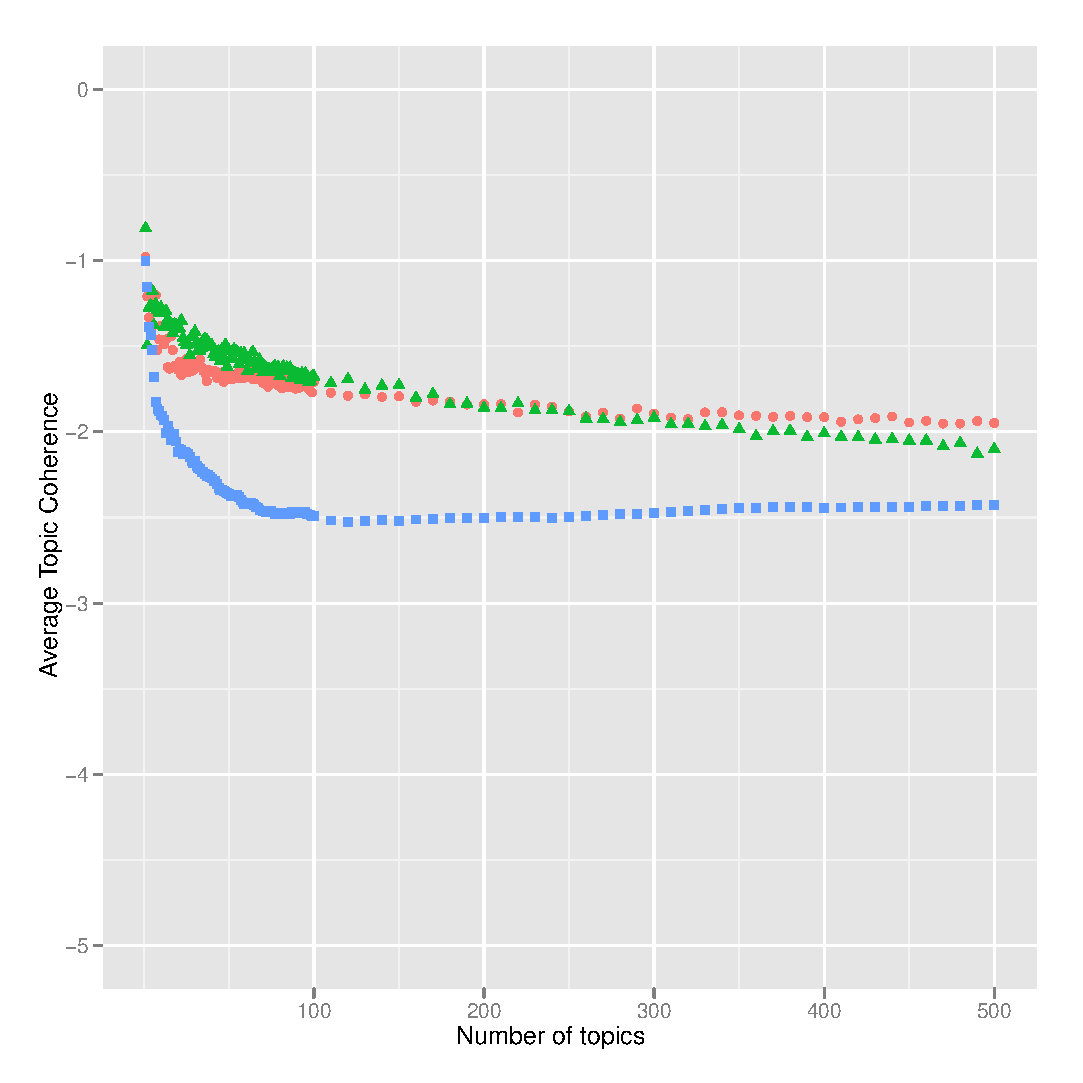
\includegraphics[width=.50\textwidth,height=.35\textwidth]{plots/mean-umass.eps}}
  \subfloat[UCI]{\label{fig:mean-uci}\includegraphics[width=.50\textwidth,height=.35\textwidth]{plots/mean-uci.eps}}
  \caption{Average Topic Coherence for each model}
  \label{fig:mean}
\end{figure*}

\begin{figure*}[h!t!b!]
  \centering
  \subfloat[UMass]{\label{fig:entropy-umass}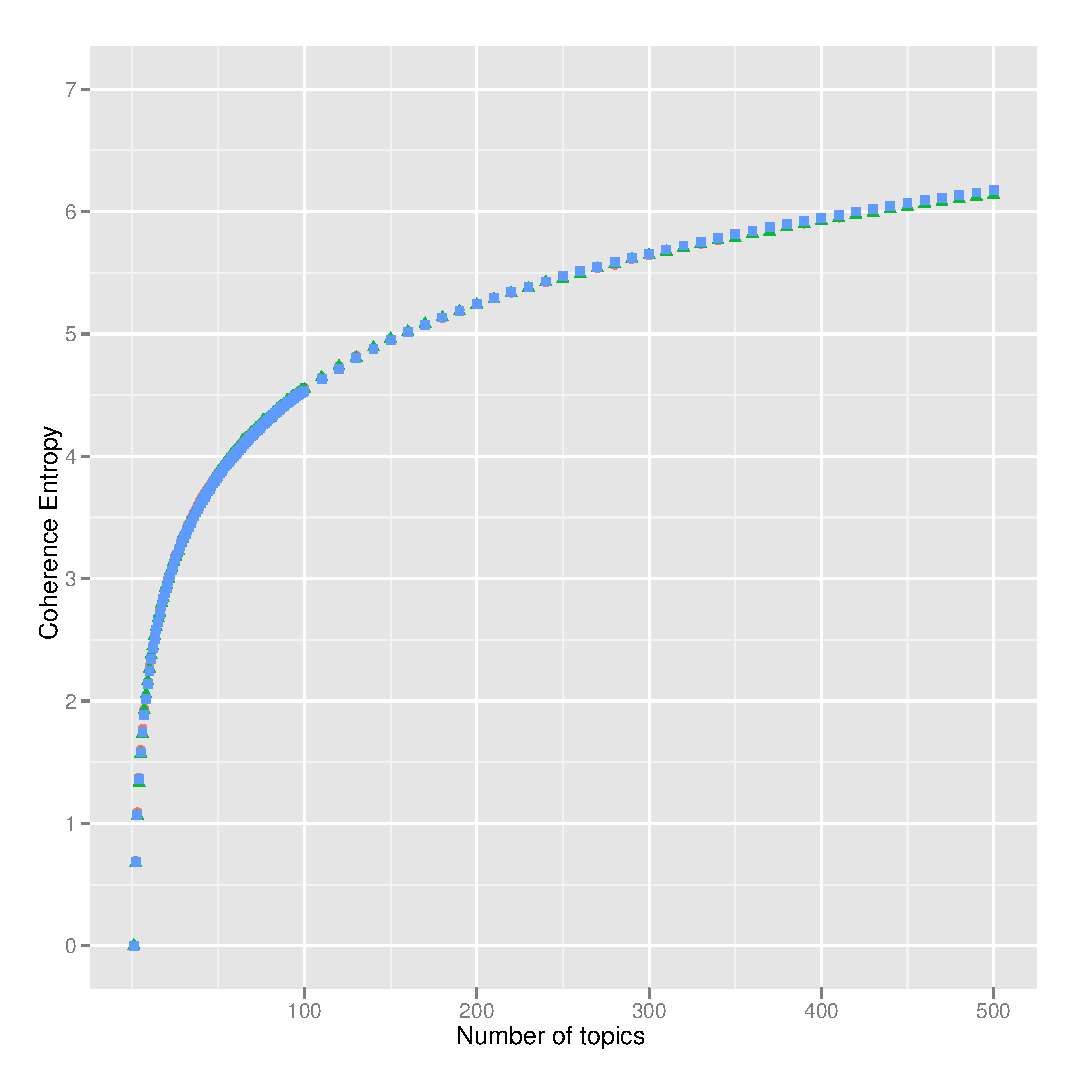
\includegraphics[width=.50\textwidth,height=.35\textwidth]{plots/entropy-umassNoLog.eps}}
  \subfloat[UCI]{\label{fig:entropy-uci}\includegraphics[width=.50\textwidth,height=.35\textwidth]{plots/entropy-uciNoLog.eps}}
  \caption{Entropy of the Topic Coherence for each model}
  \label{fig:entropy}
\end{figure*}

\paragraph{The UMass metric} defines the score to be based on document co-occurrence:

$$score(v_i, v_j,\epsilon) = \log \frac{D(v_i, v_j) + \epsilon}{D(v_j)}$$
\noindent
where $D(x,y)$ counts the number of documents containing words $x$ and $y$ and
$D(x)$ counts the number of documents containing $x$. Significantly, the UMass
metric computes these counts over the \textit{original corpus} used to train the
topic models, rather than an external corpus.  This metric is more intrinsic in
nature.  It attempts to confirm that the models learned data known to be in the
corpus.


\section{Evaluation}
\input{evaluation}

\section{Discussion and Conclusion}
\input{discussion}

\section{Acknowledgments}

This work was performed under the auspices of the U.S. Department of Energy by
Lawrence Livermore National Laboratory under Contract DE-AC52-07NA27344
(LLNL-CONF-522871) and by Sandia National Laboratory under Contract
DE-AC04-94AL85000.

\bibliographystyle{acl2012}
\bibliography{topic_coherence}

\end{document}
